\documentclass{article}
\usepackage{fullpage}
\usepackage{amsmath}
\usepackage{tikz}
\usepackage{bm}
\usepackage[hidelinks]{hyperref}
\usepackage{siunitx}

\newcommand{\Co}{C}
\newcommand{\vect}{\bm}
\newcommand{\iu}{{i\mkern1mu}}
\newcommand{\TODO}[1]{\textcolor{purple}{TODO: \emph{#1}}}

\title{Finite volume advection on spherical meshes in global Cartesian coordinates}
\author{James Shaw}

\begin{document}
\maketitle

A while ago Hilary suggested a test of zonal solid body rotation on a lat-lon mesh using a Courant number ($\Co$) of 1 and a first-order FTBS (forward-in-time, backward-in-space) scheme that should yield a perfect result.  I've been unable to achieve exactly $\Co = 1$ because there is a mismatch between face fluxes and cell volumes.  This document shows how I calculate face fluxes and explains why there is a mismatch with cell volumes.

\subsection*{Flux calculations}
In OpenFOAM, all calculations are performed in global Cartesian coordinates and all meshes are three-dimensional.  Here we consider a lat-lon spherical mesh with a single layer of cells.  We use a correction that adjusts cell volumes, cell centres, face areas and face centres that accounts for the sphericity of the mesh.

The flux at a face, $\phi$, is the integral of the wind normal to the face:
\begin{align}
	\phi = \int_f \vect{u} \cdot \vect{\hat{n}} \:df
\end{align}
where $f$ is the face area and $\vect{u}$ is the wind.  For zonal solid body rotation $\vect{u} = u_0 \cos(\theta) \vect{\hat{x}}$ where $\theta$ is a latitude and $\vect{\hat{x}}$ is a zonal unit vector.  On a lat-lon grid, fluxes are non-zero through faces that are North--South aligned.  These faces have the shape on an annular sector bounded by an inner radius $r_1$, outer radius $r_2$ and latitudes $\theta_1$ and $\theta_2$.  Integrating the wind over such a face gives

\begin{align}
	\phi &= \int_{\theta_1}^{\theta_2} \int_{r_1}^{r_2} u_0 \cos \theta r \:dr \:d\theta \\
	&= u_0 \left( \sin \theta_2 - \sin \theta_1 \right) \frac{r_2^2 - r_1^2}{2}
\end{align}
Note that $\vect{\hat{x}} \cdot \vect{\hat{n}} = 1$ for any North--South aligned face.

\subsection*{Mismatch with cell volume}
Starting with the definition of the multidimensional Courant number
\begin{align}
	\Co = \frac{\Delta t}{2 V} \sum_f \phi_f
\end{align}
On a lat-lon grid there are equal fluxes through the two North--South aligned cells:
\begin{align}
	\Co &= \frac{\Delta t}{2 V} 2 u_0 \left( \sin \theta_2  - \sin \theta_1 \right) \frac{r_2^2 - r_1^2}{2}
%
\intertext{and assuming $\Co = 1$ then}
%
	\frac{V}{\Delta t} &= u_0 \left( \sin \theta_2  - \sin \theta_1 \right) \frac{r_2^2 - r_1^2}{2}
\end{align}
However, when we calculate $V / \Delta t$ and compare it to the face fluxes we find that they are not equal: that is, the Courant number is not exactly one.  The actual Courant number varies with latitude as seen in figure~\ref{fig:Co}.

\begin{figure}
	\centering
	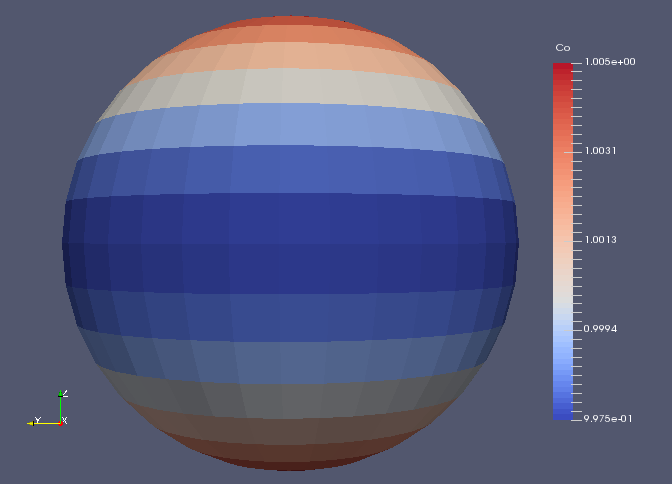
\includegraphics[width=4in]{co.png}
	\caption{Courant numbers on a coarse lat-lon mesh.  Courant numbers converge on one when the mesh is refined.}
	\label{fig:Co}
\end{figure}

\end{document}
